\chapter[Validierung]{Validierung des multimodalen Modells}\label{cha:Evaluation}
Aus gewonnen Interaktionszeiten aus Studie modellierten wir ein multimodales ein Modell, mit deren Hilfe die Dauer multimodaler Interaktionen vorhergesagt werden sollen.
Außerdem können verschiedene Kombinationen aus Modalitäten auf ihre Gesamtdauer verglichen werden. 

Im nächsten Schritt soll das erstellte multimodale Modell validiert werden. 
Dazu wollen wir in einer zweiten Studie die Gesamtdauer (Total Task Time) von multimodalen Interaktionen messen, um diese mit den Vorsagen des Modells vergleichen zu können. 

\section[Studienaufbau]{Studienaufbau}
Wir haben die Studie aufgeteilt in einen Übungsteil und den Anwendungsbeispielen, deren Gesamtdauer wir messen wollen. 
Der Übungsteil, enthält ausgewählte Anwendungsbeispiele aus Kombinationen von Modalitäten, die für den zweiten Teil benötigt werden. 
Mit diesen Übungen sollen sich die Probanden mit den Modalitäten vertraut machen. 
Im zweiten Teil sollen insgesamt fünf Anwendungsbeispiele getestet werden. Für jedes Anwendungsbeispiel wurde eine Kombination von Modalitäten festgelegt. 

Für die Auswahl der fünf Anwendungsbeispiele haben wir die Kombination von Modalitäten explizit so gewählt, dass sie in ihrer Eignung besonders gut waren siehe \fref{fig:Uebersicht_Eignung} oder deren Kombination uns interessiert hat. Die Texteingabe zum Beispiel schnitt für die Sprache deutlich besser ab, als Touch, weshalb wir diese nur mit der Modalität Sprache verwendeten. Außerdem wollen wir auch Beispiele mit mehr als einem Modalitätswechsel testen. 

Das Modell wird nur stichprobenartig validiert, um die Studie in kürzerem Rahmen zu halten. 
Das heißt, in den Anwendungsbeispielen, die wir in der zweiten Studie testen werden, kommen nicht alle modellierten Aktionen vor. 

Die Studie zur Validierung unseres Modells fand unter gleichen Bedingungen erneut bei BMW in Garching-Hochbrück am Parkring 19 in der Parkgarage im gleichen Studienfahrzeug (BMW 6er Gran Coupé) statt. 
Das Auto wurde ans Stromnetz angeschlossen, um das Surface zu laden und eine Dauerhafte Stromversorgung für Licht sowie Sitzheizung zu ermöglichen.
Das Surface wurde erneut am Dashboard und der Leap Motion Controller zwischen Gangschaltung und Dashboard angebracht. Die Einstellungen, der Aufbau des Prototypen, sowie die Protokollierung wurde wie in der ersten Studie vorgenommen. 

Die Einverständniserklärung, sowie den demographischen Fragebogen verwendeten wir gleichermaßen wie in der ersten Studie. 

Um in dieser Studie zusätzlich die subjektive Beanspruchung der Interaktionen zu messen, wurde der NASA Task Load Index (kurz NASA TLX) nach jedem Anwendungsbeispiel abgefragt \ref{cha:Anhang}. 
Der NASA TLX bewertet die subjektive Beanspruchung und unterscheidet dabei 6 Kategorien (Geistige Anforderung, Körperliche Anforderung, Zeitliche Anforderung, Leistung, Anstrengung und Frustration), die bewertet werden. 
Nach den 5 Anwendungsbeispielen wurde der zweite Teil des NASA TLX abgefragt, bei dem alle 6 Beanspruchungsvarianten miteinander verglichen. 
Die 15 Vergleiche wurden für jeden Probanden in unterschiedlicher Reihenfolge abgefragt, um mögliche Einflüsse zu vermeiden. 
Außerdem wurde am Ende der Studie der INTUI Fragebogen abgefragt, um die Usability des Prototypen einzuschätzen. 
Sowie drei Fragen in einem weiteren Fragebogen siehe \ref{cha:Anhang}. 
  
In den folgenden Unterabschnitten werden die Übungsbeispiele und die Anwendungsbeispiele erläutert. 
\subsection[Übungsbeispiele]{Übungsbeispiele der Validierungsstudie}
Bevor wir mit den Anwendungsbeispielen für die Evaluation beginnen, soll in der Evaluationsstudie erst geübt werden. 
Dafür verwenden wir die Variante des Prototypen aus der ersten Studie. 
Die Anwendungsbeispiele sind dort kürzer und so können sich die Probanden mit den Interaktionen vertraut machen.
Wir haben folgende Übungsvarianten aus der ersten Studie gewählt (siehe \fref{fig:UseCases}):
\begin{enumerate}
	\item Navigation (Modalität: Geste und Sprache)
	\item Lautstärke (Modalität: Geste und Touch)
	\item Lautstärke (Modalität: Sprache und Geste)
	\item Temperatur (Modalität: Sprache und Touch)
	\item Telefon (Modalität: Touch und Sprache)
	\item Telefon (Modalität: Geste und Touch)
\end{enumerate}
Mit diesen Übungsbeispielen wurde die Direktauswahl aus sichtbaren Elementen (DA) mit Geste, Sprache und Touch geübt. Die Listennavigation (L) mit Sprache und Touch. Die direkte Inkrementation (Inkr. (d)) des Sliders mit Touch und Geste und zuletzt die schrittweise Inkrementation (Inkr.(s)) der Temperatureinstellung mit Touch. Das sind alle Interaktionen, die wir evaluieren wollen. 
\subsection[Anwendungsbeispiele]{Anwendungsbeispiele der Validierungsstudie}
Nach diesem Übungsdurchgang sollen fünf Anwendungsbeispiele getestet werden. 
Dafür passen wir den multimodalen Prototypen etwas an.
 
Im Anwendungsbeispiel "`Lüftung"' soll die Lüftung auf Stufe 3 gestellt werden (siehe \fref{fig:UseCasesEvalLuft}). Dafür muss zuerst die Lüftungskachel mit dem Sprachbefehl "`Lüftung"' selektiert werden. 
Anschließend wird mit drei Swipe-Touchgesten die Lüftung von null auf drei gestellt. 
Der Wert wird nach einer kurzen Pause von selbst eingeloggt, es muss also nicht bestätigt werden.  
\begin{figure}
	\centering
		\includegraphics[width=1\textwidth]{img/UseCases_Eval_Luft.jpg}
	\caption[]{Anwendungsbeispiel Lüftung mit den Modalitäten Sprache und Touch}
	\label{fig:UseCasesEvalLuft}
\end{figure}
Die Vorhersage der Interaktionsdauer mit dem multimodalen Modell wird folgendermaßen berechnet:
\[
\textbf{Lüftung} = \text{DA}_\text{S} + R(DA) + V(\text{Inkr.} (s))_\text{T} + 3*\text{Inkr.} (s)_\text{T}  + W_\text{ST} + R(\text{Screen}) =
\]
\[
= 2,795\text{s} + 0,5\text{s} + 0,906\text{s} + 3*0,547\text{s} +  0,273\text{s} + 0,016\text{s} = 6,133\text{s}
\]

Das Anwendungsbeispiel "`Lautstärke"' kennen wir bereits aus der ersten Studie. 
Es soll die Lautstärke von 50\% auf 80\% erhöht werden, mit den Modalitäten Sprache und Geste, siehe \fref{fig:UseCasesEvalMedienS}. 
Zuerst wird mit den Sprachbefehlen "`Medien"' und "`Lautstärke"' zweimal die Aktion Direktauswahl aus sichtbaren Elementen ausgeführt. 
Anschließend wird mit der direkten Inkrementation die Lautstärke verstellt. 
\begin{figure}
	\centering
		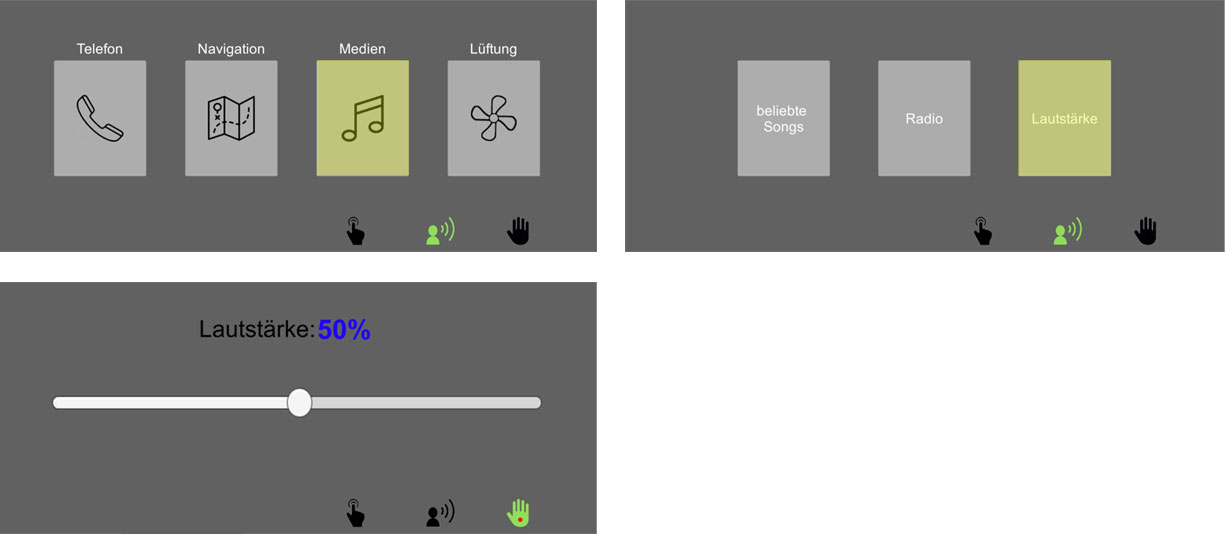
\includegraphics[width=1\textwidth]{img/UseCases_Eval_MedienS.jpg}
	\caption{Anwendungsbeispiel Lautstärke mit den Modalitäten Sprache und Touch}
	\label{fig:UseCasesEvalMedienS}
\end{figure}
Die Berechnung zur Vorhersage der Interaktionsdauer mit unserem Modell sieht wie folgt aus:
\[
\textbf{Lautstärke} = 2*(\text{DA}_\text{S} + R(DA)) + \text{Inkr.} (d)_\text{G} + W_\text{SG} + 3*R(\text{Screen}) =
\]
\[
= 2*( 2,795\text{s} + 0,5\text{s}) + 4,593\text{s} + 0,127\text{s} + 3*0,016\text{s} = 11,358 \text{s}
\]

Im Anwendungsbeispiel "`Medien"' soll zunächst per Geste die DA die Kachel "`Medien"' und "`beliebte Songs"' ausgewählt werden. 
Es erscheint eine Liste mit beliebten Songs. 
Mit dem Sprachbefehl "`Happy"' wird das Lied Happy abgespielt. 
Auf dem nächsten Screen, soll mit Touch die Lautstärke geändert werden. 
Dafür wird per Touch der Lautstärke Button selektiert. 
Es erscheint ein Slider, der von 20\% auf 80\% ebenfalls per Touch geändert werden soll. 
Wird der Slider im Bereich von 75 und 85\% losgelassen kommt ein Popup, dass noch per Touch bestätigt werden muss, siehe \fref{fig:UseCasesEvalMedien}.
\begin{figure}
	\centering
		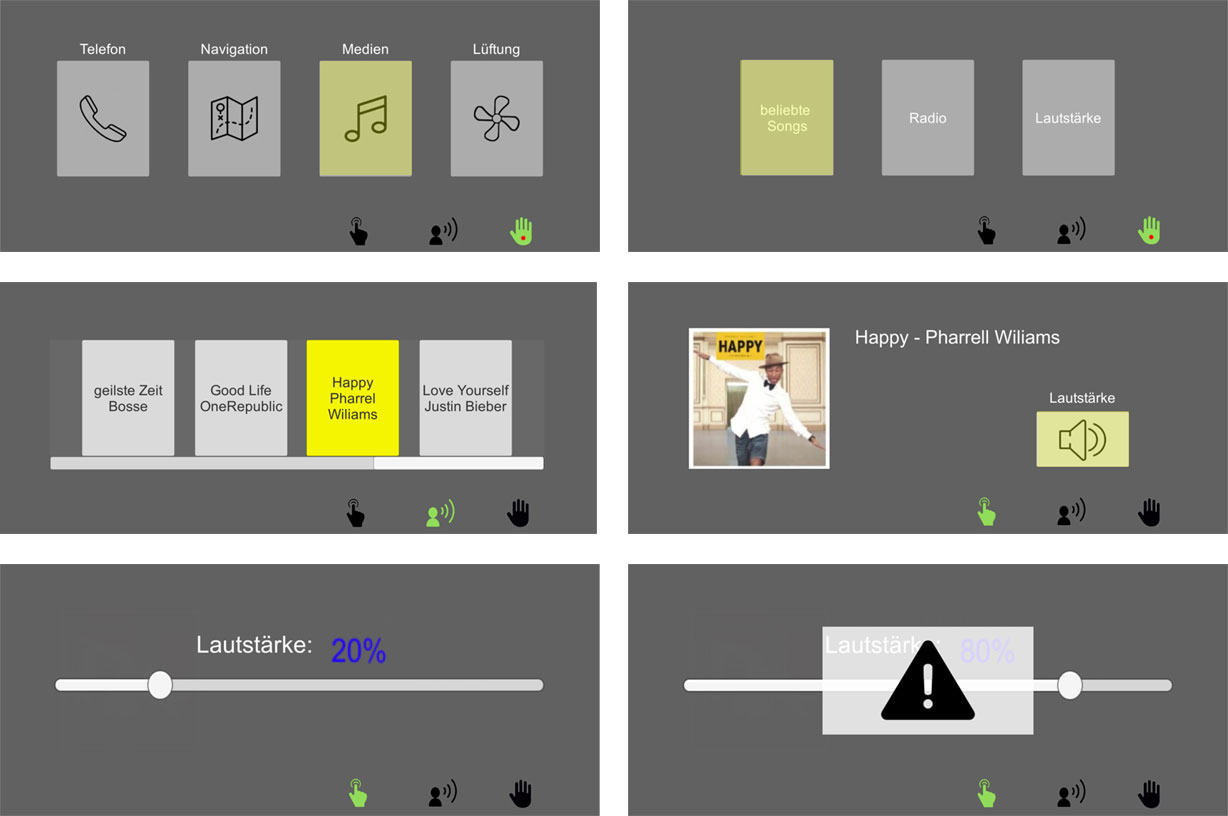
\includegraphics[width=1\textwidth]{img/UseCases_Eval_Medien.jpg}
	\caption{Anwendungsbeispiel Lautstärke mit den Modalitäten Geste, Sprache und Touch}
	\label{fig:UseCasesEvalMedien}
\end{figure}
Die Interaktionszeit besteht aus diesen Aktionszeiten und Wechselkosten:
\[
\textbf{Medien} = 2*(\text{DA}_\text{G}) + \text{Wort(m)}_\text{S} + W_\text{GS} + V(\text{1. Bu.})_T + \text{1-3 Bu.} + W_\text{ST} + 
\]
\[
 + Inkr.(d)_\text{T} + B_\text{T} + 6*R(\text{Screen}) =
\]
\[
= 2*( 2,436\text{s}) + 2,839\text{s} + 0,105\text{s} + 1,123\text{s} + 1,495\text{s} + 0,218\text{s} +
\]
\[
+2,795\text{s}+0,829\text{s} + 6*(0,016) = 15,014\text{s}
\]

Im Anwendungsbeispiel "`Navi POI"' wollen wir mit den Modalitäten Geste, Sprache und Touch den nächsten Coffeeshop finden. 
Dazu werden per Geste die Kacheln "`Navigation"' und "`Points of Interest"' ausgewählt. 
Dann erscheint ein Texteingabefeld mit einem Inputfeld zur Eingabe des POI. 
Mit dem Sprachbefehl "`Fastfood"' wird Fastfood in das Inputfeld eingetragen. 
Erneut mit Spracheingabe wird die Eingabe mit "`OK"' bestätigt. 
Jetzt wechselt der Screen zu einer Liste von Fastfood Geschäften. 
Es muss zum Starbucks auf der zweiten Seite mit der Touch-Eingabe geswiped werden. 
Auf der dritten Seite angekommen, muss noch die Starbuckskachel ausgewählt werden, siehe \fref{fig:UseCasesEvalNaviPOI}.  
\begin{figure}
	\centering
		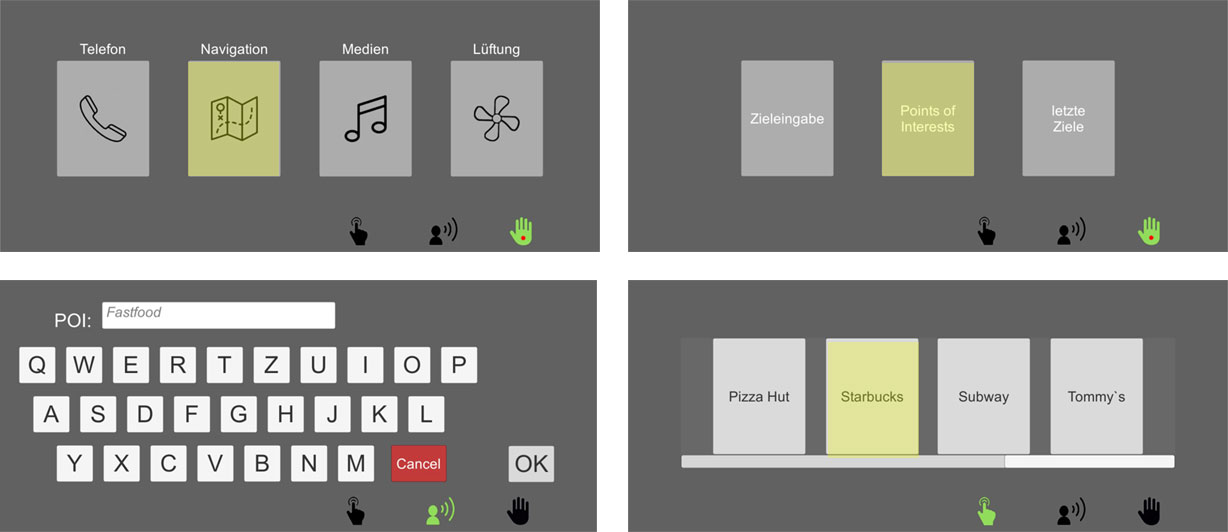
\includegraphics[width=1\textwidth]{img/UseCases_Eval_Navi_POI.jpg}
	\caption{Anwendungsbeispiel Navihation POI mit den Modalitäten Geste, Sprache und Touch}
	\label{fig:UseCasesEvalNaviPOI}
\end{figure}

In der ersten Studie haben wir festgestellt, dass die Positionierung des Inputfeldes über der Tastatur besser geeignet ist, da somit die Hand nicht die Eingabe verdeckt. Obwohl in unserer Kombination keine Touch-Eingabe verwendet wird, haben wir diese Anpassung bei den Screens mit Texteingabe vorgenommen.

Die Aktionsdauer dieses Anwendungsbeispiels wird folgendermaßen zusammengesetzt und berechnet:
\[	
\textbf{Navi POI} = 2*(\text{DA}_\text{G}) + \text{Wort(m)}_\text{S} + W_\text{GS} + B_\text{S} + 
\]
\[	
+ V(\text{L})_T + 2*(L)_T + W_\text{ST}(L_T) + DA(L)_T + 4*R(\text{Screen}) =
\]
\[
= 2*( 2,436\text{s}) + 2,839\text{s} + 0,105\text{s} + 1,972\text{s} + 
\]
\[
= + 0,705\text{s} + 2*0,813\text{s} + 1,495\text{s} + 0,375\text{s} + 1,047\text{s} + 4*0,016= 13,605\text{s}
\]

Im Anwendungsbeispiel "`Navigation Nummer"' soll zum Parkring 19 navigiert werden. Hier werden 2 Modalitäten (Touch und Sprache) mit insgesamt vier Moduswechseln verwendet. Per Touch werden die Kacheln Navigation und Zieleingabe gedrückt. 
Es wird das Texteingabefeld mit zwei Inputfeldern (Straße und Nummer) geladen. 
Um das Inputfeld "`Straße"' zu aktivieren, muss auf das Straße-Inputfeld getapt werden. 
Mit dem Sprachbefehl "`Parkring"' wird die Straße in das Inputfeld eingetragen. 
Anschließend wird erneut mit einem Tap auf das Nummer-Inputfeld, dieses aktiviert. 
Mit dem Sprachebefehl "`19"' wird die 19 in das Inputfeld eingetragen. 
Als letztes wird mit der Touch-Eingabe das Ziel mit dem OK-Button bestätigt, siehe (\ref{fig:UseCasesEvalNaviNummer}).
\begin{figure}
	\centering
		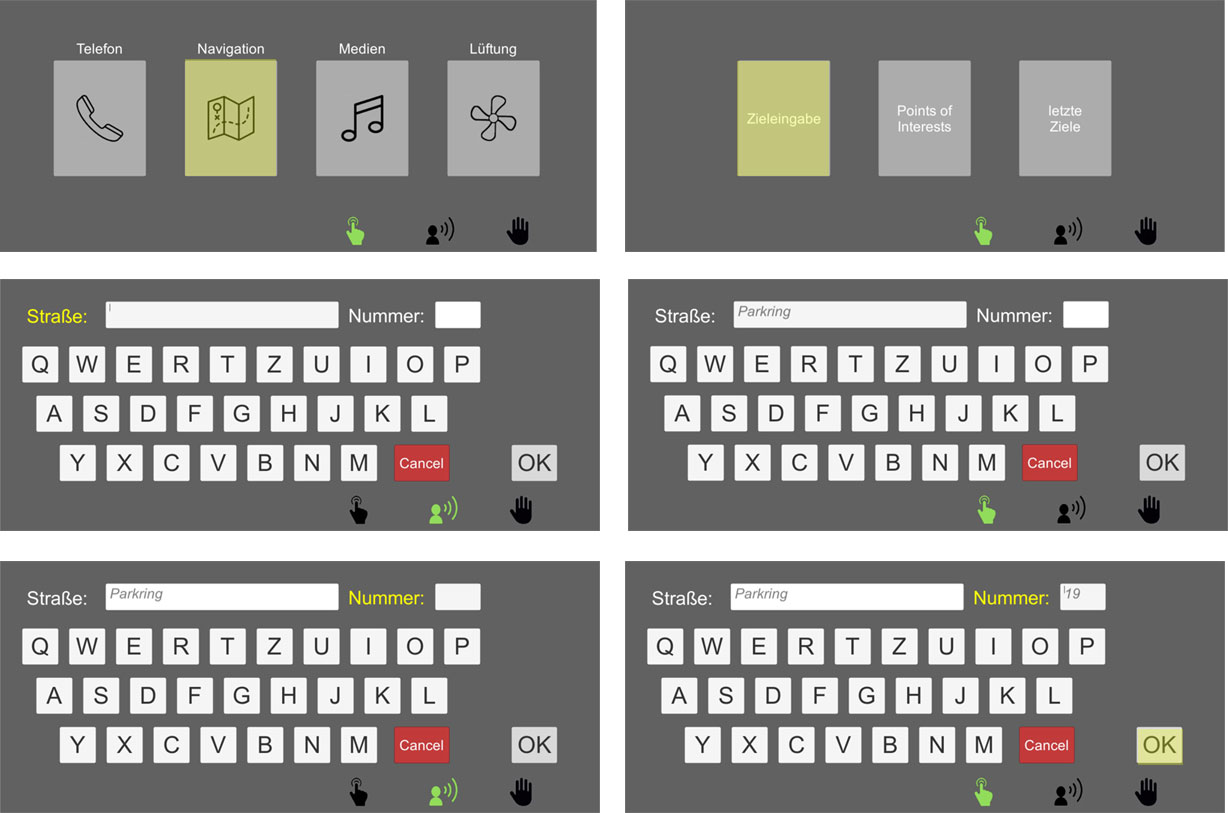
\includegraphics[width=1\textwidth]{img/UseCases_Eval_Navi_Nummer.jpg}
	\caption{Anwendungsbeispiel Navihation POI mit den Modalitäten Touch, Sprache, Touch, Sprache, Touch}
	\label{fig:UseCasesEvalNaviNummer}
\end{figure}	
Auch hier berechnen wir mit dem erstellten Modell die Interaktionsdauer. Sie setzt sich aus diesen Aktionszeiten und Wechselkosten zusammen:
\[
\textbf{Navi Nummer} = 2*(\text{DA}_\text{T}) + V(\text{1. Bu.})_T + \text{1-3 Bu.}_T + \text{Wort(m)}_S + W_\text{TS}(Wort(m)) +
\]
\[
+ V(\text{1. Bu.})_T + \text{1-3 Bu.}_T + W_\text{ST}(1. Bu.) + \text{Wort(m)}_\text{S} + W_\text{TS} + B_\text{T} + W_\text{ST} + 4*R(\text{Screen}) =
\]
\[
= 2*( 1,710\text{s}) +  1,123\text{s} + 0,642\text{s} + 2,839\text{s} + 0,079\text{s} + 1,123\text{s} + 
\]
\[
+ 0,642\text{s} + 0,218\text{s} + 2,839\text{s} + 0,079\text{s} + 0,642\text{s} + 1,123\text{s} + 0,218\text{s} + 3*0,016 = 15,035\text{s}
\]

\section[Studiendesign]{Studiendesign}
Wie in der ersten Studie zur Erhebung von Interaktionszeiten, verwenden wir in der Validierungsstudie ebenfalls ein Within Subject Design, indem jeder Proband alle fünf Anwendungsbeispiele durchführen wird. 
Von jedem der Anwendungsbeispiele werden erneut zwei Messdurchgänge vorgenommen. 
Nach jedem Messdurchgang wurde die Eignung des Anwendungsbeispiel abgefragt und ob das Anwendungsbeispiel dem Probanden gefallen hat.

Die 5 Anwendungsbeispiele wurden mit dem Latin Square permutiert, um auch in dieser Studie mögliche Lerneffekte zu eliminieren. Die Übungsbeispiele zu Beginn eines Studiendurchlaufs wurden jedoch in gleicher Reihenfolge durchlaufen. 

Diese Vorhersage der Interaktionsdauer für unsere 5 Anwendungsbeispiele wird die Grundlage unserer Validierung sein. 
Wir werden die Zeiten Anwendungsbeispiele messen und mit unseren Vorhersagen vergleichen. 

\section[Studienteilnehmer]{Studienteilnehmer}
Die Studiendauer eines Durchgangs betrug ca. 45 Minuten. In einem Zeitraum von zwei Tagen nahmen an der Evaluationsstudie insgesamt 10 Teilnehmer (8 männlich und 2 weiblich) teil. Das Alter erstreckte sich von 19-33 Jahren und betrug im Durchschnitt 23,8 mit einen Median von 22 Jahren, also etwas jünger als in unserer ersten Studie (Durchschnitt: 30,55 und Median: 25 Jahre). Alle 10 Teilnehmer sind Rechtshänder und sprechen deutsch als Muttersprache. 

Auch in der Evaluation wurde die Vorerfahrungen mit der Bedienung von Touch, Gesten und Sprache der Teilnehmer abgefragt und von den Probanden eingeschätzt. Auf die Frage, ob sie Erfahrung mit der Bedienung von Sprache, Touch und Geste haben, konnte aus vier Optionen gewählt werden (1: nein, 2: ja, aber nur sehr wenig, 3: ja, benutze ich gelegentlich und 4: ja, benutze ich regelmäßig). Die Vorerfahrung der Bedienung von Sprache ergab im Durchschnitt 3,1, bei Touch 4 und bei Geste 2,2. Die Werte sind etwas besser als in unserer ersten Studie (Sprache: 2,32,  Touch: 3,95 und Geste: 1,86), was unter anderem daran liegen könnte, dass die Teilnehmer etwas jünger waren.

\section[Durchführung der Studie]{Durchführung der Studie}
Auch in dieser Studie wurde jeder Proband am Empfang am Parkrings 19 abgeholt und begrüßt.
Anschließend begaben wir uns in die Parkgarage zum Testfahrzeug, indem der Proband auf dem Fahrersitz platz nehmen sollte.
Er wurde darauf hingewiesen das Smartphone lautlos zu stellen und den Fahrersitz einzustellen.

Das Thema der Studie wurde kurz erläutert und darauf aufmerksam gemacht, dass zur Erhebung der Interaktionszeiten verschiedene Daten protokolliert werden und zusätzlich die Studie mit einer GoPro aufgezeichnet wird.
Darüber aufgeklärt musste jeder Proband eine Einverständniserklärung unterschreiben (siehe Kapitel \ref{cha:Anhang}).
Zusätzlich sollte ein kurzer Fragebogen zu demografischen Daten und den Vorerfahrungen zum Umgang mit den Interaktionen Touch, Geste und Sprache ausgefüllt werden.
In der Zwischenzeit startete der Studienleiter das Programm, stellte die richtige ID ein und überprüfte die neu geladene Permutation.

Die Vorgehensweise wurde Schritt für Schritt anhand der 6 Übungsbeispiele erklärt und somit konnten sich die Probanden mit den Interaktionen vertraut machen. 
Anschließend wurde die GoPro-Kamera gestartet, um die kommenden Anwendungsbeispiele für die Messung aufzunehmen.
Bei jedem Anwendungsbeispiel wurde zusätzlich in einem Probedurchlauf mindestens einmal der Vorgang geübt. 

Anschließend konnte mit dem ersten Messdurchgang begonnen werden. 
Nach jedem Messdurchgang wurde auch in dieser Studie auf einer 5-stufigen Likert-Skala abgefragt, wie geeignet die Probanden die Interaktion empfanden und wie sehr sie ihnen gefallen hat.
Traten während eines Messdurchgangs Fehler auf, wurde das vom Versuchsleiter notiert, um den Protokolleintrag im Nachhinein als fehlgeschlagen markieren zu können. 
Dieser Messdurchgang wurde dann wiederholt. 
Als fehlerhaft wurde ein Messdurchgang gewertet wenn zum Beispiel die Touch-, Gesten- oder Spracherkennung nicht richtig funktionierte oder wenn der Proband vergaß was er tun muss. 

\section[Auswertung der Studienergebnissen]{Auswertung der Studienergebnissen}
Im folgenden werden nun die Ergebnisse der Evaluationsstudie präsentiert und diskutiert. 


\subsection{Ergebnisse des Modells}
Um unsere vorhergesagten Zeiten mit den beobachteten Zeiten vergleichen zu können berechnen wir mit dem Root Mean Square Error (RMSE). Er wird wie folgt berechnet, wobei r unsere beobachteten Zeiten pro Proband (residuals) sind und p die vorhergesagten Zeiten.
\[
RMSE = \sqrt{\frac{1}{n}\sum_{i=1}^{n}(r_i - p_i)^2}
\]
Der RMSE gibt uns an wie viele Sekunden die beobachteten Zeiten durchschnittlich von unserer Vorhersage abweichen. Uns interessiert der prozentuale Fehler, also wird der RMSE noch durch unsere vorhergesagte Zeit geteilt. Wir verwenden eine logarithmische Skala, um die vorhergesagten Zeiten unseres Modells mit den beobachteten Zeiten aus der Evaluation darzustellen, da der Fehler proportional zur Dauer sein soll \citep{Card_1980} und \citep{schneegass_2009}. 

Die \fref{fig:predictedVsObserveredData} zeigt, dass sich unsere vorhergesagten Zeiten sehr gut mit den beobachteten Zeiten decken. 
\begin{figure}
	\centering
		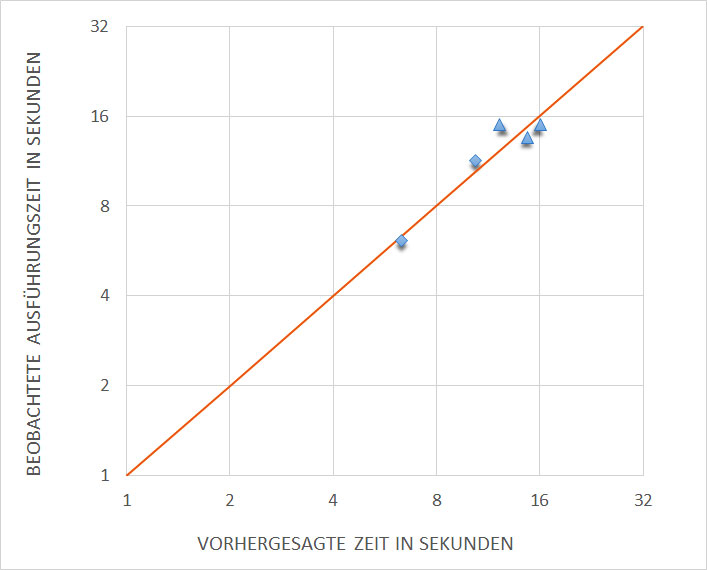
\includegraphics[width=1\textwidth]{img/predictedVsObserveredData.jpg}
	\caption[Übersicht der 5 Aufgaben im Vergleich zu den vorhergesagten und beobachteten Zeiten]{Übersicht der 5 Aufgaben im Vergleich zu den vorhergesagten und beobachteten Zeiten. Die Rauten sind Aufgaben mit nur einem Moduswechsel im Stil der ersten Studie. Die Dreiecke sind die Anwendungsbeispiele mit 2 und 4 Moduswechseln.}
	\label{fig:predictedVsObserveredData}
\end{figure}

Der Durchschnittliche RMSE der 5 Anwendungsbeispiele beträgt 14,746\%, was deutlich geringer ist als die maximale Erwartung von 20-30\% \citep{Card_1980} und generell ganz gut im Bereich von 5\% -20\% liegt \citep{Luo_2005}, \citep{Teo:2006}. Da unser Modell nicht ganz so feingranulare Unterscheidungen macht wie beim KLM und deren Erweiterungen war auch ein größerer Vorhersagefehler zu erwarten. Deshalb ist der durchschnittliche Vorhersagefehler von 14,746\% eine ziemlich gute Annäherung der multimodalen Interaktionszeit. 

In der \fref{tab:PredictedVsObserved} können die vorhergesagten Zeiten, der beobachteten Durchschnittszeiten, der RMSE in Sekunden und prozentual, sowie der durchschnittlichen Belastung des NASA TLX entnommen werden. 
\begin{table}[ht]
  \centering
		\begin{tabular}{|l|l|l|l|l|l|}
				\hline
				Aufgabe			& vorhergesagte 	& durchschnittliche 	& RMSE	& RMSE 		& Beanspruchung\\
				Modi (Wechsel)	& Zeit (s) 				& Zeit (s)						& (s)		& (\%) 		& NASA TLX 	 \\
				\hline
				Lüftung 			& 6,132						& 6,326 (+0,194)								& 0,864	&	14,098	&	25,600\\
				S,T (1)				&& 						&	&		&	\\
				\hline
				Lautstärke	& 11,36						&	10,413 (-0,947)							& 1,614 &	14,202	&	29,700\\
				S,G (1)				&& 						&	&		&	\\
				\hline
				Medien				& 15,014 					&	16,016 (+1,002)							& 1,860	&	12,389	&	33,100\\	
				G,S,T (2)			&& 						&	&		&	\\
				\hline
				Navi POI			& 13,605					& 14,682 (+1,077)							& 1,685	& 12,385	& 32,067\\
				G,S,T (2)			&& 						&	&		&	\\
				\hline
				Navi Nummer		& 15,035					& 12,215	(-2,82)						& 3,105 & 20,654	& 37,533\\		
				T,S (4)				&& 						&	&		&	\\
				\hline	
			\end{tabular}
	\caption[Vorhergesagte Werte im Vergleich zu beobachteten Werten]{Vorhergesagte Werte im Vergleich zu beobachteten Werten, deren RMSE in Sekunden und prozentual, sowie die durchschnittliche Beanspruchung des NASA TLX (Skala von 0-100)}
	\label{tab:PredictedVsObserved}
\end{table}

Unser Modell scheint auch für Interaktionen mit mehr als einem Moduswechsel anwendbar zu sein. Gerade die Vorhersage der Anwendungsbeispiele Medien und Navi POI mit je 3 verschiedenen Modalitäten und somit 2 Modalitätswechsel ergeben die besten Ergebnisse mit einer Fehlerabweichung von nur 12,39\%. 

Die kompletten Ergebnisse aller 10 Probanden dieser beiden Anwendungsbeispiele sind in \fref{fig:Medien_Times} und \fref{fig:Navi_POI_Times} zu sehen. 

Bei dem Anwendungsbeispiel Medien liegt die Durchschnittszeit der Probanden über der vorhergesagten Zeit. Ein Grund dafür kann sein, dass für die Erhebung der Aktion Inkr. (d) eine Verschiebung von 50\% auf das Interval 75-85\% gemessen wurde. In dem Evaluationsbeispiel sollte die Lautstärke von 20\% auf das Interval von 75-85\% gestellt werden. Da hier die Spanne größer ist, könnte dieser Teil etwas länger gedauert haben. 

Auch beim Anwendungsbeispiel Navi POI lag die vorhergesagte Zeit unter dem Durchschnitt. 
\begin{figure}
			\centering
			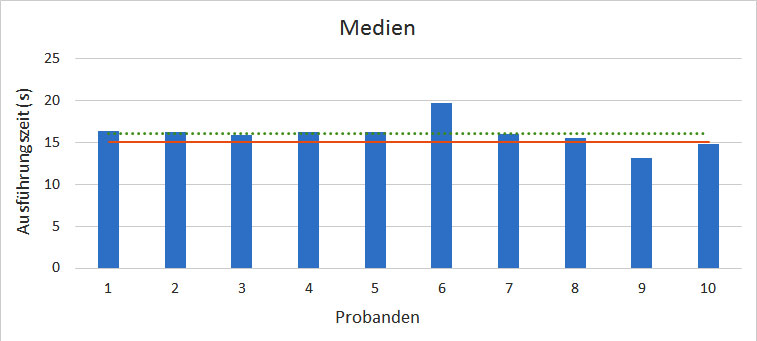
\includegraphics[width=1\textwidth]{img/Medien_Times.jpg}
			\caption[Zeiten der Probanden für das Anwendungsbeispiel Medien.]{Zeiten der Probanden für das Anwendungsbeispiel Medien. Enthält Modalitäten Geste, Sprache und Touch. Die rote durchgehende Linie stellt die vorhergesagte Zeit dar, die grüne gepunktete die Durchschnittszeit aller Probanden.}
			\label{fig:Medien_Times}
\end{figure}
\begin{figure}
			\centering
			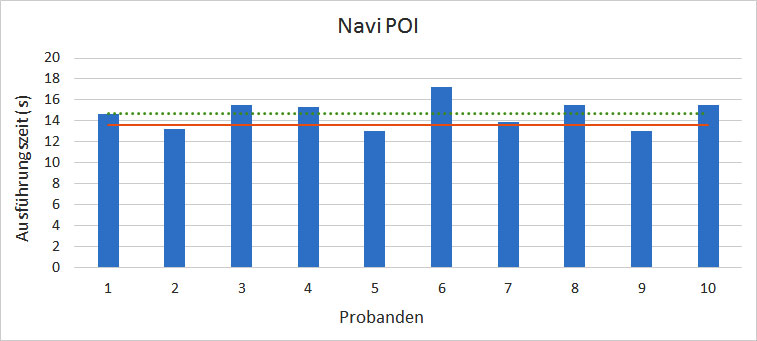
\includegraphics[width=1\textwidth]{img/Navi_POI_Times.jpg}
			\caption[Zeiten der Probanden für das Anwendungsbeispiel Navigation zu POI.]{Zeiten der Probanden für das Anwendungsbeispiel Navigation zu POI. Enthält Modalitäten Geste, Sprache und Touch. Die rote durchgehende Linie stellt die vorhergesagte Zeit dar, die grüne gepunktete die Durchschnittszeit aller Probanden.}
			\label{fig:Navi_POI_Times}		
\end{figure}

Die Anwendungsbeispiele Lüftung und Lautstärke waren fast identisch zu Beispielen aus der ersten Studie. Die hatten beide nur einen Moduswechsel. Beim Anwendungsbeispiel Lüftung liegt unsere Vorhersage unter dem Durchschnitt. Das Anwedungsbeispiel Lautstärke liegt allerdings unsere Vorhersage über dem Durchschnitt. 
Das ist eventuell der Tatsache zu schulden, dass die Probanden der Evaluationsstudie insgesamt besser mit der Slidegeste für die Einstellung des Lautstärkesliders zurecht kamen. 
Die kompletten Ergebnisse aller 10 Probanden dieser beiden Anwendungsbeispiele sind in den \ref{fig:Luft_Times} und \ref{fig:MedienS_Times} zu entnehmen. 
\begin{figure}
			\centering
			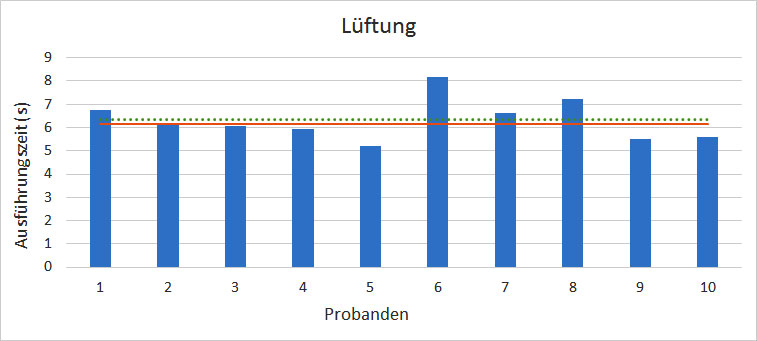
\includegraphics[width=1\textwidth]{img/Luft_Times.jpg}
			\caption[Zeiten der Probanden für das Anwendungsbeispiel Lüftung.]{Zeiten der Probanden für das Anwendungsbeispiel Lüftung. Enthält Modalitäten Sprache und Touch. Die rote durchgehende Linie stellt die vorhergesagte Zeit dar, die grüne gepunktete die Durchschnittszeit aller Probanden.}
			\label{fig:Luft_Times}
\end{figure}
\begin{figure}
			\centering
			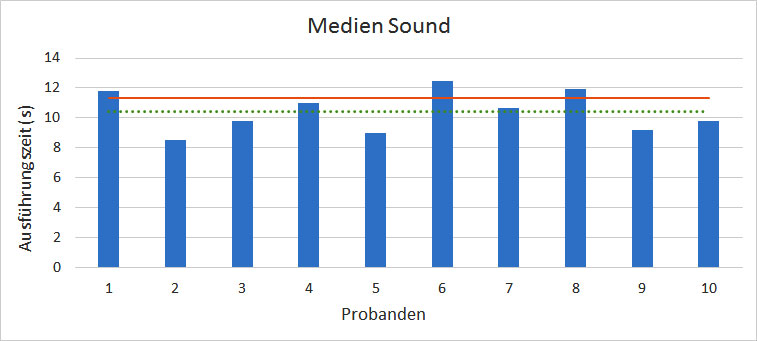
\includegraphics[width=1\textwidth]{img/Medien_S_Times.jpg}
			\caption[Zeiten der Probanden für das Anwendungsbeispiel Lautstärke.]{Zeiten der Probanden für das Anwendungsbeispiel Lautstärke. Enthält Modalitäten Sprache und Geste. Die rote durchgehende Linie stellt die vorhergesagte Zeit dar, die grüne gepunktete die Durchschnittszeit aller Probanden.}
			\label{fig:MedienS_Times}		
\end{figure}

Das Anwendungsbeispiel Navi schnitt am schlechtesten ab mit einem prozentualen RMSE von 20,654\%. Mit zwei verschiedenen Modalitäten und vier Moduswechseln ist dies das aufwändigste Beispiel. Für die Aktivierung der Inputfelder verwendeten wir in unserem Modell zur Vorhersage die Zeit den ersten Buchstaben zu drücken. Im Beispiel ist die Touchfläche allerdings deutlich größer als die Touchfläche der Buchstaben aus unserer ersten Studie. Nach Fitts` Law \citep{fitts1954information}, \citep{sasangohar2009evaluation}
beeinflusst die Größe der Touchfläche W die Interaktionszeit positiv. Es erschien es uns besser die Interaktionszeit zu überschätzen, als zu unterschätzen. Es lässt sich in diesem Beispiel gut erkennen, das unsere Vorhersage für alle Probanden zu groß waren siehe \fref{fig:Navi_Times}.
\begin{figure}
	\centering
		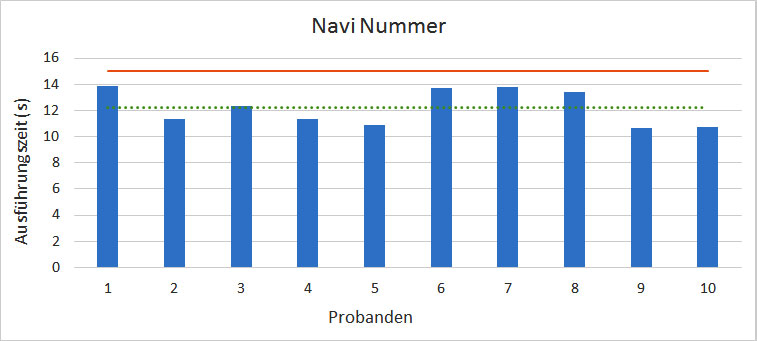
\includegraphics[width=1\textwidth]{img/Navi_Times.jpg}
	\caption[Zeiten der Probanden für das Anwendungsbeispiel Navigation.]{Zeiten der Probanden für das Anwendungsbeispiel Navigation. Enthält Modalitäten Touch, Sprache, Touch, Sprache und Touch. Die rote durchgehende Linie stellt die vorhergesagte Zeit dar, die grüne gepunktete die Durchschnittszeit aller Probanden.}
	\label{fig:Navi_Times}
\end{figure}
\subsection{Vergleich des Modells ohne Wechselkosten}

\subsection[User Experience]{User Experience}
Im Vergleich zu Touch und Sprache war für die Teilnehmer die Gestensteuerung am ungewohntesten. 
Die Einschätzung der Eignung der Anwendungsbeispiele mit Geste schnitt nicht so gut ab wie die Anwendungsbeispiele ohne Geste. Allerdings bekam im Anwendungsbeispiel Lautstärke, indem der Lautstärkeslider mit einer Geste verstellt werden sollte, sehr positives Feedback siehe \ref{fig:Smiley_Eignung_Gefallen}. Es wurde auf die Frage, ob Ihnen die Interaktion gefallen würde nur eine negative Antwort gegeben. Nach jedem Messdurchgang (also 2 pro Anwendungsbeispiel) sollten die Probanden auf einer Likertskala mit 5 Unterscheidungen angeben wie geeignet sie die Anwendung fanden und ob es Ihnen gefallen hat.
\begin{figure}
	\centering
		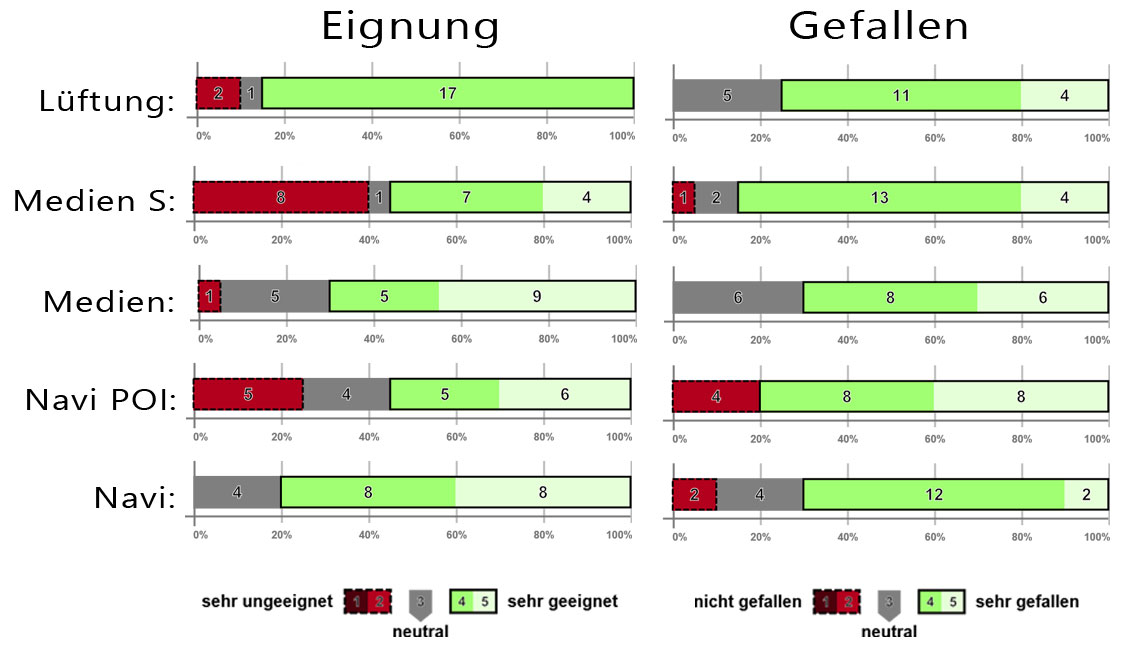
\includegraphics[width=1\textwidth]{img/Smiley_Eignung_Gefallen.jpg}
	\caption[Eignung und Gefallen der 5 Aufgaben]{Eignung und Gefallen der 20 Messdurchgänge der 5 Aufgaben. Die Balkendiagramme zur Darstellung von Likert-Skalen wurde mit http://likertplot.com/ generiert.}
	\label{fig:Smiley_Eignung_Gefallen}
\end{figure}
 
9 von 10 Teilnehmern können sich eine multimodale Interaktion während dem Fahren vorstellen. Begründungen waren die intuitive Bedienung, sowie vor allem der Vorteil sich je nach Situation die passende Modalität frei wählen zu können.

Im INTUI Fragebogen (siehe Anhang im Kapitel \ref{cha:Anhang}) werden verschiedene Komponenten der intuitiven Nutzung auf einer Skala von 1-7 abgefragt \citep{diefenbach2010handbuch}, \citep{ullrich2010intui}. Die Probanden wurden hierfür darauf hingewiesen, dass sie sich dafür unseren Prototypen fehlerfrei vorstellen sollten. Denn unsere Umsetzung des Prototypen ist natürlich kein vollständig ausgearbeitetes Produkt.  
Die 17 Fragen mit verschiedenen Gegenüberstellungen werden vier Hauptbereichen zugewiesen (siehe \citep[Seite 24]{diefenbach2010handbuch}):
\begin{itemize}
	\item \textbf{Mühelosigkeit (M):} Je höher der Wert, um so müheloser wird die Interaktion erlebt und desto weniger Aufmerksamkeit wird erfordert.  Diese Komponente kann am ehesten mit der klassischen Usability verglichen werden.
\item \textbf{Bauchgefühl (G):} Je höher der Wert, um so weniger wird die Interaktion vom Verstand, sondern vom Gefühl geleitet. Diese Komponente ist "`eines der wichtigsten Merkmale intuitiver Entscheidungen in der Entscheidungspsychologie sowie im alltäglichen Sprachgebrauch"'\citep[Seite 24]{diefenbach2010handbuch}.
\item \textbf{Magisches Erleben (X):} Je faszinierender und außergewöhnlicher die Interaktion empfunden wurde desto höher ist der Wert. 
\item \textbf{Verbalisierungsfähigkeit (V):} Je höher der Wert, desto besser kann die Interaktion beschrieben werden. 
\end{itemize}
Die Ergebnisse des INTUI Fragebogens können aus \fref{fig:INTUI} entnommen werden.
\begin{figure}
	\centering
		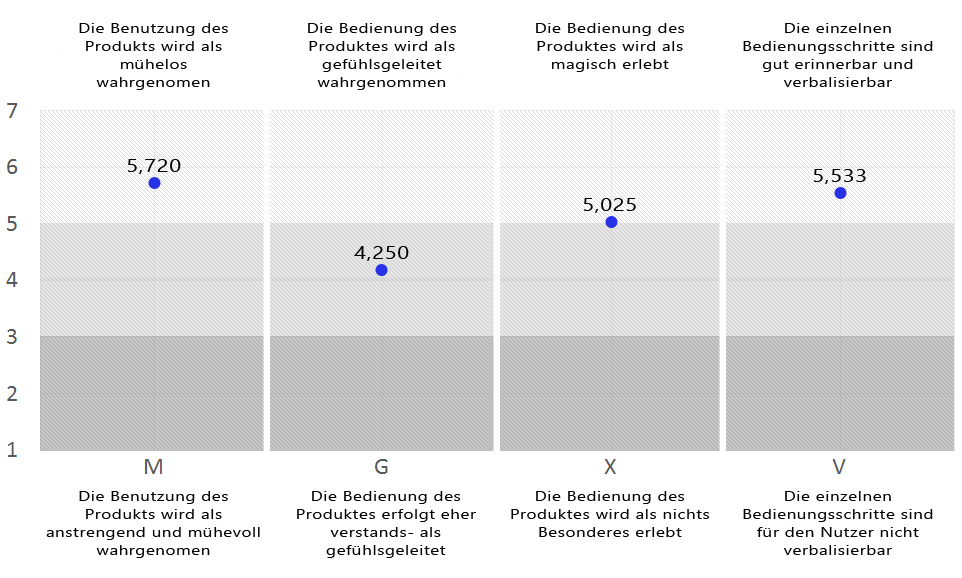
\includegraphics[width=1\textwidth]{img/INTUI_Grafik.jpg}
	\caption{Mittelwerte der 4 Komponenten des INTUI Fragebogens}
	\label{fig:INTUI}
\end{figure}
Der extremste Wert ist mit 5,72 bei der Mühelosigkeit. Das deutet auf eine gute Usability unseres Prototypen hin. Beim Bauchgefühl zeigt der Wert eine minimale Tendenz zu einer gefühlsgeleitenden Interaktion hin. Der Wert des Magischen Erlebens mit 5,025 deutet  auf eine außergewöhnliche Interaktion hin. Die Abfolge unserer Bedienschritt schien unseren Probanden als einleuchtend, zumindest befindet sich der Wert der Verbalisierungsfähigkeit mit 5,533 im oberen Bereich.

\subsection{subjektive Belastung}
Beim NASA Task Load Index mussten 6 Beanspruchungskriterien auf einer Skala von 1-20 subjektiv von den Probanden bewertet werden. Diese Werte werden alle mit 5 multipliziert, um eine Abstufung von 1-100 zu erhalten. 

Im zweiten Teil werden alle Kriterien miteinander verglichen und mit diesen 15 Vergleichen werden jetzt die Kriterien gewichtet. Wurde die Frustration 4 mal vorgezogen erhält die Frustration eine Gewichtung (G) von 4. Die Bewertung wird also mit 5 und dann mit deren Gewichtung multipliziert. All diese Werte aufsummiert durch 15 geteilt ergeben den gesamten NASA TLX. Diese Gewichtung führt dazu, dass für den Nutzer unwichtige Kriterien weniger bis gar nicht miteinbezogen werden und dafür wichtige um so mehr. 

Sei $B$ die Menge der Beanspruchungen, im speziellen Geistige Anforderung, Körperliche Anforderung, Zeitliche Anforderung, Leistung, Anstrengung und Frustration, dann sieht die Berechnung wie folgt aus:
\[
\textbf{NASA TLX} =\frac{1}{15}\sum_{i \in B}A_{i}G_{i}
\]
wobei $A_i$ der Wert der Beanspruchung ist und $G_i$ die Gewichtung.

Der durchschnittliche NASA TLX jedes Anwendungsbeispiels ist aus der \fref{tab:PredictedVsObserved} zu entnehmen. Das Anwendungsbeispiel Lüftung verursachte mit einem Wert von 25,6 die geringste Beanspruchung. Am meisten beanspruchte das Anwendungsbeispiel Navi Nummer mit den 4 Moduswechseln mit einem Wert von 37,533.
Wir stellen fest, dass mit Dauer der vorhergesagten Interaktionzeiten auch die durchschnittliche Beanspruchung zunimmt.
\section[Diskussion]{Diskussion}
Die Evaluierung unseres multimodalen Modells soll nun mit Hinblick auf die Ergebnisse diskutiert und mit Ergebnissen aus anderen Arbeiten verglichen werden. Des Weiteren gehen wir auf qualitative Erkenntnisse ein, die sich aus beiden Studien durch Kommentare und Beobachtungen ergeben haben.

\subsection[Modell]{Multimodales Modell}
Die fünf evaluierten Anwendungsbeispiele ließen sich mit unserem Modell mit einem durchschnittlichen RMSE von 14,746\% vorhersagen. Dieser durchschnittliche RMSE befindet sich sowohl im Bereich von 20-30\% den \citet{Card_1980} als maximalen Fehler empfiehlt, als auch im Bereich von 5-20\% \citep{Luo_2005}, \citep{Teo:2006}. \citet{Card_1980}, \citet{Luo_2005} und \citet{Teo:2006} bewerten allerdings ein Keystroke-Level-Modell oder deren Erweiterung auf Operatorebene. Davon ausgehend, dass unser Modell wesentlich grobgranularer aufgebaut ist als das Keystroke-Level-Modell, stellt sich unser Modell zur Vorhersage von multimodalen Interaktionen als vielversprechend heraus. 

\citet{Teo:2006} erklärt, dass es zwei Nachteile bei der Verwendung der gesamten Aufgabendauer gibt. 
Zum einen inkorrekte Messungen und falsch gesetzte Operatoren. 
In unserem Modell haben wir verschiedene Aktionen je nach Modalität und deren Wechselkosten modelliert. 
Eine Aktion enthält allerdings, anders als bei den bisherigen Keystroke-Level Modellen auch mehrere Operatoren. 
Dies macht unser Modell etwas gröber, allerdings ist die Platzierung der Aktionen einfacher. 
Nimmt ein Nutzer die Hand zum Beispiel einmal mehr zurück zum Lenkrad, ist dies kein Fehler, sondern hängt von der Situation ab. 
Diese Unterschiede in der Ausführung der Aktionen steckt in unseren Zeiten mit drinnen. 
Deshalb halten wir die gesamte Dauer der Interaktion für ein geeignetes Maß für den Vergleich. 

Die subjektive Bewertung der Nutzer durch den NASA TLX Ihrer Beanspruchung während der multimodalen Interaktion lag zwischen 25,6 und 37,533 auf einer Skala von 0-100. Den durchschnittlichen Beanspruchungswert von 25,6 hatte das Anwendungsbeispiel Lüftung mit den Modalitäten Sprache und Touch mit einem Moduswechsel. Es lässt sich erkennen, dass die Beanspruchung mit der vorhergesagten Interaktionsdauer zunahm bis zum Wert von 37,533 im Anwendungsbeispiel Navi Nummer. Dieses Anwenungsbeispiel stellte sich mit insgesamt 4 Moduswechseln der Modalitäten Touch und Sprache als das mit der größten Beanspruchung heraus. (Paper mit vergleichbaren Ergebnissen). 

Diese Beanspruchungswerte scheinen in Ordnung zu sein, denn 9 von 10 Teilnehmern können sich eine multimodale Interaktion im Stile unserer Evaluationsstudie während dem Fahren vorstellen. Die intuitive Bedienung, sowie dem Vorteil sich je nach Situation die passende Modalität frei wählen zu können kommt bei den Nutzern gut an. Jedoch bleibt in diesem Feld der multimodalen Interaktion noch viel zu forschen und entwickeln bis die Erwartungen und Vorteile vollends ausgeschöpft werden können.

Beispielsweise haben wir in unserer Evaluation nicht alle Aktionen mit allen Modalitäten evaluiert. Mit 1,5 Stunden dauerte die erste Studie sehr lange und es konnte beobachtet werden, dass die Konzentration mit der Zeit etwas nach ließ. Die Evaluationsstudie wollten wir dementsprechend kürzer gestalten. 

Außerdem haben wir uns speziell Anwendungsbeispiele für die Evaluationsstudie herausgesucht, die uns möglichst realistisch in der Anwendung erschienen. Die Bewertung der Nutzer auf die Eignung der Interaktionen und wie gut sie Ihnen gefallen hat schnitt ganz gut. Das lässt darauf hindeuten, dass unsere Wahl zutreffend war, siehe \fref{fig:Smiley_Eignung_Gefallen}.
Die Texteingabe per Touch wurde nicht evaluiert, da die Spracheignung deutlich besser eingeschätzt wurde. Ebenso die Aktion Inkr. (d) und Inkr. (s) wurde für die Gesteninteraktion nicht evaluiert. 

Die beliebtesten Moduskombinationen der 22 Nutzer aus der ersten Studie waren die unimodale Variante mit Sprache. Am zweit beliebtesten war die Kombination von Touch und Sprache. Die dritt beliebteste Variante war die Kombination von Geste und Sprache. 

Das Design unseres Prototypen wurde Anhand der im Workshop (Connected Minds) gewonnenen Informationen über Interaktionen im Auto modelliert. Wir mussten uns auf bestimmte Gesten einigen, die uns am sinnvollsten erschienen für unsere Aktionen erschienen. Es gibt jedoch andere Varianten, die ebenfalls als Aktionen in Frage kommen. Zum Beispiel die kreisförmige Geste mit dem Zeigefinger nach links oder rechts, um die Lautstärke zu verringern oder zu erhöhen. Eine Geste dieser Art ist bereits im BMW 7 Series eingebaut. Die Implementierung mit der Leap Motion dieser Geste war mit der neuen Version von Unity nicht so einfach umsetzbar, weshalb wir uns dort eine andere Variante überlegten.

Ein weiterer Mangel unseres Modell sind, wie schon erwähnt, die fehlenden haptischen Bedienelemente. Diese sind natürlich ein wichtiger Bestandteil und sollte als weitere Modalität in unser Modell miteinbezogen werden. 

Bei der Aktion Inkr. (d) wurde in der ersten Studie zur Erhebung der Interaktionszeiten lediglich der Slider von 50\% auf 75-85\% verstellt. Für unsere grobe Betrachtung erschien uns diese Einstellung als ausreichend zur Bestimmung dieser Interaktionszeit. Da in dem Anwendungsbeispiel der Evaluation jedoch die Zeiten für eine Verstellung von 20 auf 75-85\% länger dauerte, sollte diese Aktion eventuell genauer untersucht werden. 

\subsection[Qualitative Erkenntnisse]{Qualitative Erkenntnisse}
Während beider Studien zur Bedienung eines multimodalen Interface im Auto ist aufgefallen, dass der Bereich von Gesteninteraktionen sehr individuell von der Sitzeinstellung und Armlänge abhängt. Am ergonomisch geeignetsten hatten es die Nutzer, die ihren Arm an der Armlehne ablegen konnten und sich trotzdem mit der Hand im gewünschten Interaktionsbereich befanden. 

Für zukünftige Gestensteuerung im Auto sollte das berücksichtigt werden, um verkrampfte und unnatürliche Bewegungen zu reduzieren. Zum Beispiel könnte durch eine verstellbare Armlehne, sowie einen anpassbaren Interaktionsbereich zur Gestenerkennung die optimale Einstellung erreicht werden. Das ermöglicht nicht nur eine bequemere Gesteninteraktion, sondern reduziert auch mögliche Erkennungsfehler von Gesten, was wiederum zu einer besseren User Experience führt.

Der Touchbereich war ebenfalls für manche Nutzer nur gut zu Erreichen, indem sie sich etwas vor lehnten. Sie  wurden angewiesen sich vor der Studie den Sitz so einzustellen als würden sie fahren, doch trotz diesen Vorkehrungen war der Touchdisplay nicht für alle optimal positioniert. Auch in der Touchbedienung gibt es noch Potenzial zur Verbesserung. Die Erreichbarkeit des Touchbereichs sollte weiter vorne gelegen sein, als bei Informationssystemen im Auto ohne Touchdisplays.